\section{Querschnittliche Konzepte}

\subsection{LoL Database ER-Diagram}
\graphic{LoLDatabase}{ER-Diagramm der LoL Datenbank}
In dieser Datenbank werden alle League of Legends bezogenen Daten gespeichert. Das sind alle Daten die dann auch im Frontend angezeigt werden. Die Daten werden vom Games Importer Service in die Datenbank geschrieben und dann von der Player API für das Frontend zur Verfügung gestellt.\\
Tabellen in der Datenbank:\\
\begin{itemize}
\item \textbf{Summoners:} Daten für einen Spieler
\item \textbf{Games:} Daten für einzelne Spiele
\item \textbf{Challenges:} Werte des Spieler in einer Challenge
\item \textbf{ChallengeClasses:} Verschiedene Challenges, die in der Challenges Tabelle auftauchen können, mit genauerer Beschreibung und Einteilung in Klassen
\item \textbf{SummonerSpells:} Klasse für Mapping von SummonerSpell IDs zu Name und Icon URL
\item \textbf{Champions:} Klasse für Mapping von Champion IDs zu Name und Icon URL
\item \textbf{Items:} Klasse für Mapping von Item IDs zu Name und Icon URL
\item \textbf{SummonerIcons:} Klasse für Mapping von Icon IDs zu URL
\item \textbf{Patches:} Hier wird gespeichert, welche Patches von League of Legends bereits in der Datenbank eingetragen wurden. Da mit jedem Patch z.B. neue Icons dazukommen, müssen die Tabellen nach jedem Patch geupdated werden. Nach dem update wird in dieser Tabelle festgehalten, wann die Datenbank für welchen Patch geupdated wurde.
\end{itemize}

\subsection{User Database ER-Diagramm}
\todo{User DB ER-Diagram}

\subsection{User Management API Spezifikation}
\todo{User Management API Spec}

\subsection{Player API Spezifikation}
\todo{Player API Spec}

\subsection{GRPC Interface}
Damit der Import eines neuen Spieler angefragt werden kann, muss eine Kommunikation zwischen Frontend und dem Games Importer Service bestehen. Das Frontend kommuniziert nur mit der PlayerAPI, welche die Anfrage dann an den Games Importer Service weiterleiten muss.\\
Da der Player API Service und der Games Importer Service beide in Pyton geschrieben wurden, kann diese Kommunikation über GRPC erfolgen, welches es der PlayerAPI erlaubt über einen Protocol Request die Import Funktion des Game Importers aufzurufen.\\ % TODO Tim: für grps müssen Applikationen nicht in gleicher Sprache geschrieben sein. Grund war eher, dass grpc Streaming erlaubt
Die Schnittstelle wird in einer .proto Datei definiert:

\begin{lstlisting}
syntax = "proto3";

service Importer {
  rpc import_player (ImportRequest) returns (stream ImportReply) {}
}

message ImportRequest {
  string puuid = 1;
}

message ImportReply {
  int32 games_imported = 1;
  int32 total_games = 2;
}
\end{lstlisting}
Der Request beinhaltet hierbei die ID des zu importierenden Spielers und die Reply den aktuellen Fortschritt des Vorgangs. Die Reply wird solange gesendet, bis der Spieler vollständig importiert wurde.\\
Mithilfe dieser Datei werden dann die nötigen Python Klassen generiert. In der \textit{PlayerImportRequest.py} wird dann die \textit{import\_player(request, context)} Methode implementiert, welche dann beim erhalten eines Requests aufgerufen wird und im request Parameter die ID des Spieler erhält. Dann kann der Games Importer diesen importieren und mittels eines \textit{yield} Statements in der \textit{import\_player()} Funktion die Replies an die Player API senden.

\subsection{Zentrales Logging}

Um das Debuggen im Fehlerfall zu vereinfachen gibt es es zentrales Logging.
Die Logs aller Services werden zentral von Loki eingesammelt und gespeichert.
Die Logs werden über ein Docker Plugin direkt an Loki gesendet.
Über Grafana lassen sich die Logs mit der Query Sprache Logql durchsuchen.
So können zum Beispiel alle Logs eines Accounts im Games Importer Service angezeigt werden:

\begin{lstlisting}
  {compose_service="riot-api-connector"} |= `'accountId': 'P90cNvGn`
\end{lstlisting}

Das Ergebnis ist in Abbildung~\ref{fig:logging} zu sehen.
Oben wird auf einer Zeitachse dargestellt, wann, wie viele Logs gefunden werden.
Darunter sind alle gefundenen Logzeilen zu sehen.
Logzeilen können ausgeklappt werden, um weitere Metainformationen zu sehen.

\begin{figure}
    \centering
    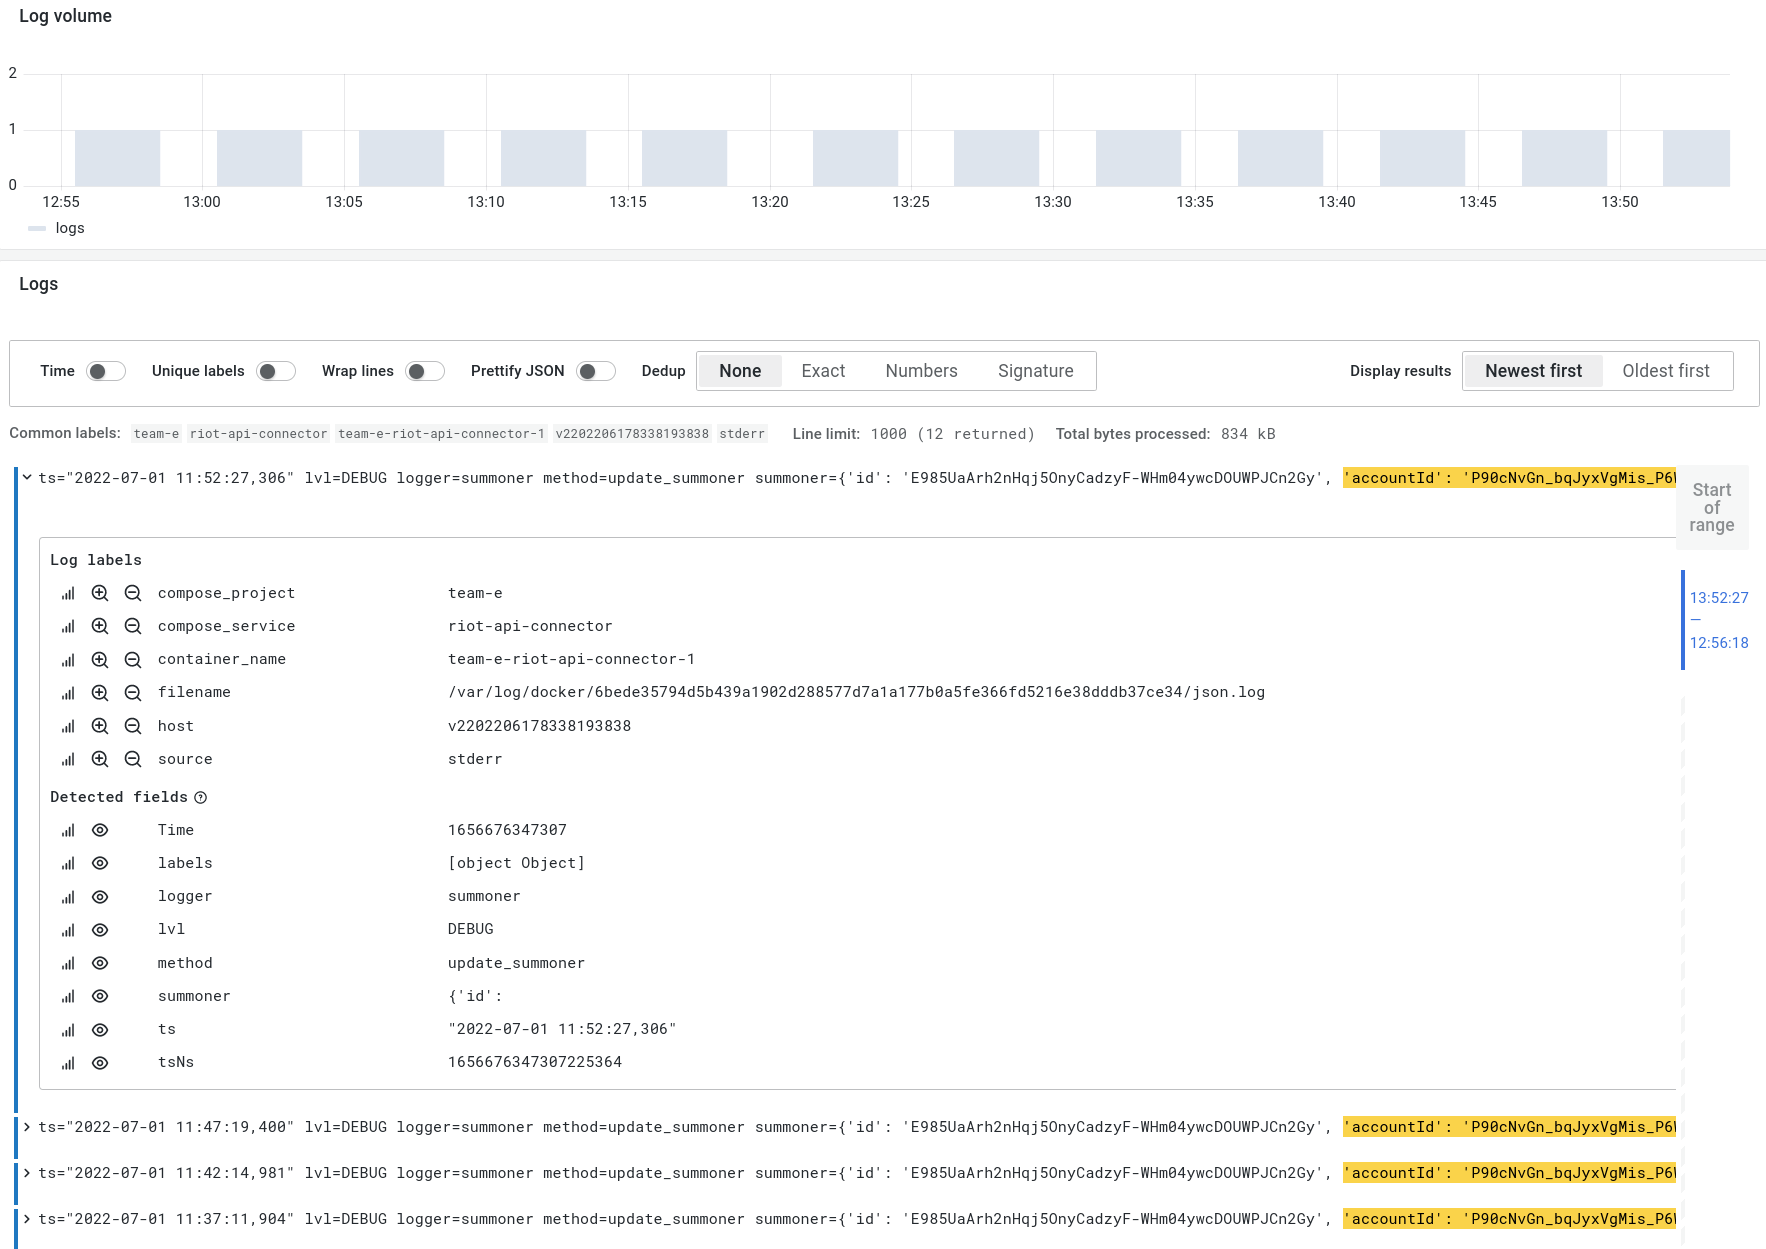
\includegraphics[width=\textwidth]{images/logging}
    \caption{Ergebnis des Logging Queries}
    \label{fig:logging}
\end{figure}